\section{Classification using Nearest Neighbour}
This chapter will give information on the classification method called k-Nearest Neighbour (k-NN).

The NN is shortly "given a collection of data point and query points in an m-dimentional metric space, find the data point that is closets to the query point"
\citep{meaningfulNN}.

This means that the NN classification will need a dataset that can train a system \citep{Sinyor05}, the data used for training has to be annotated so that the program that makes the classification knows what the different data represent. 
Once the data has been acquired and trained, it will need to be measured against the value-description. This is because difference in pronunciation and method can make it difficult for the computer to differentiate. A solution to this is to use make use of different features to describe the variation. \\

When a test-sound is to be classified, a feature vector is calculated using the same features and feature parameters as used when training the k-NN.
The euclidean distance is then calculated between the test-feature vector and all the train-feature vectors \citep{NNHD}.
The k will then be how many neighbours that has to be compared at before determining what the new input is, then the most represented sound will be chosen and labelled as the class of the input sound \citep{introKNN}.

\begin{figure}[h]
	\begin{center}
		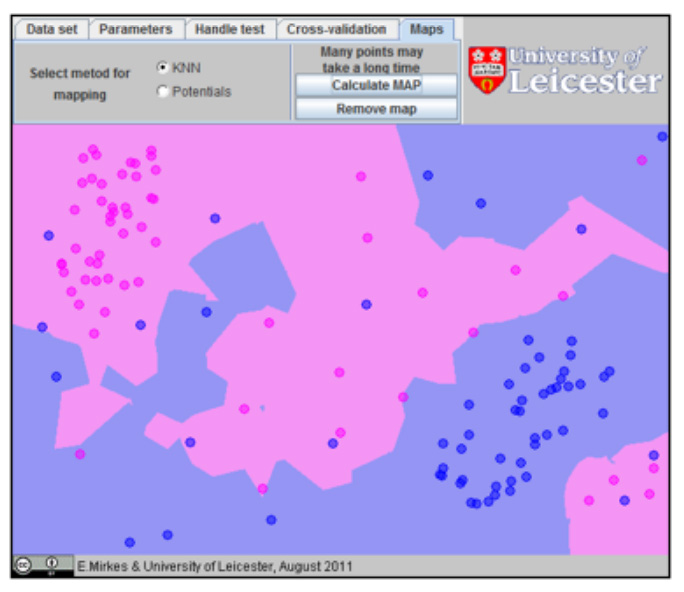
\includegraphics[scale = 0.5]{fig/KNNfig.jpg}
		\caption{Illustration of how k-NN will divide the space up with to different classes \citep{introKNN}}
		\label{KNN fig}
	\end{center}
\end{figure}

\colorbox{red}{OUR IMPLEMENTATION WILL BE DESCRIBED HERE (STILL NEEDED!!)}